\documentclass[chi_draft]{sigchi}

% Use this section to set the ACM copyright statement (e.g. for
% preprints).  Consult the conference website for the camera-ready
% copyright statement.

% Copyright
\CopyrightYear{2017}
%\setcopyright{acmcopyright}
\setcopyright{acmlicensed}
%\setcopyright{rightsretained}
%\setcopyright{usgov}
%\setcopyright{usgovmixed}
%\setcopyright{cagov}
%\setcopyright{cagovmixed}
% DOI
\doi{} %http://dx.doi.org/10.475/123_4}
% ISBN
\isbn{} %123-4567-24-567/08/06}
%Conference
\conferenceinfo{IoT'17,}{October 22--25, 2017, Linz, Austria}
%Price
\acmPrice{\$15.00}

% Use this command to override the default ACM copyright statement
% (e.g. for preprints).  Consult the conference website for the
% camera-ready copyright statement.

%% HOW TO OVERRIDE THE DEFAULT COPYRIGHT STRIP --
%% Please note you need to make sure the copy for your specific
%% license is used here!
% \toappear{
% Permission to make digital or hard copies of all or part of this work
% for personal or classroom use is granted without fee provided that
% copies are not made or distributed for profit or commercial advantage
% and that copies bear this notice and the full citation on the first
% page. Copyrights for components of this work owned by others than ACM
% must be honored. Abstracting with credit is permitted. To copy
% otherwise, or republish, to post on servers or to redistribute to
% lists, requires prior specific permission and/or a fee. Request
% permissions from \href{mailto:Permissions@acm.org}{Permissions@acm.org}. \\
% \emph{CHI '16},  May 07--12, 2016, San Jose, CA, USA \\
% ACM xxx-x-xxxx-xxxx-x/xx/xx\ldots \$15.00 \\
% DOI: \url{http://dx.doi.org/xx.xxxx/xxxxxxx.xxxxxxx}
% }

% Arabic page numbers for submission.  Remove this line to eliminate
% page numbers for the camera ready copy
% \pagenumbering{arabic}

% Load basic packages
\usepackage{balance}       % to better equalize the last page
\usepackage{graphics}      % for EPS, load graphicx instead 
\usepackage[T1]{fontenc}   % for umlauts and other diaeresis
\usepackage{txfonts}
\usepackage{mathptmx}
\usepackage[pdflang={en-US},pdftex]{hyperref}
\usepackage{color}
\usepackage{booktabs}
\usepackage{textcomp}

% Some optional stuff you might like/need.
\usepackage{microtype}        % Improved Tracking and Kerning
% \usepackage[all]{hypcap}    % Fixes bug in hyperref caption linking
\usepackage{ccicons}          % Cite your images correctly!
% \usepackage[utf8]{inputenc} % for a UTF8 editor only

% Custom packages

\usepackage{paralist}

\usepackage{tikz}
\usetikzlibrary{shadows,shapes}
\usepackage{pgfplots}
\pgfplotsset{compat=1.10}

\usepackage{xcolor}
\usepackage{colortbl}
\definecolor{Gray}{gray}{0.90}

\usepackage{algorithm}
\usepackage{algorithmicx}
\usepackage{algpseudocode}

% If you want to use todo notes, marginpars etc. during creation of
% your draft document, you have to enable the "chi_draft" option for
% the document class. To do this, change the very first line to:
% "\documentclass[chi_draft]{sigchi}". You can then place todo notes
% by using the "\todo{...}"  command. Make sure to disable the draft
% option again before submitting your final document.
\usepackage[textsize=small]{todonotes}
\newcommand{\TODO}[1]{\todo[inline]{#1}}

\newcommand{\field}[1]{\texttt{#1}}

% Paper metadata (use plain text, for PDF inclusion and later
% re-using, if desired).  Use \emtpyauthor when submitting for review
% so you remain anonymous.
\def\plaintitle{Private Blockchains for Transactive Energy:\\Security, Privacy, and Safety}
\def\plainauthor{First Author, Second Author, Third Author}
\def\emptyauthor{}
\def\plainkeywords{Internet of Things; blockchain; transactive energy; privacy; security; transactive microgrid.}
\def\plaingeneralterms{Design, Human Factors, Reliability, Security} % TODO: revise

% llt: Define a global style for URLs, rather that the default one
\makeatletter
\def\url@leostyle{%
  \@ifundefined{selectfont}{
    \def\UrlFont{\sf}
  }{
    \def\UrlFont{\small\bf\ttfamily}
  }}
\makeatother
\urlstyle{leo}

% To make various LaTeX processors do the right thing with page size.
\def\pprw{8.5in}
\def\pprh{11in}
\special{papersize=\pprw,\pprh}
\setlength{\paperwidth}{\pprw}
\setlength{\paperheight}{\pprh}
\setlength{\pdfpagewidth}{\pprw}
\setlength{\pdfpageheight}{\pprh}

% Make sure hyperref comes last of your loaded packages, to give it a
% fighting chance of not being over-written, since its job is to
% redefine many LaTeX commands.
\definecolor{linkColor}{RGB}{6,125,233}
\hypersetup{%
  pdftitle={\plaintitle},
% Use \plainauthor for final version.
%  pdfauthor={\plainauthor},
  pdfauthor={\emptyauthor},
  pdfkeywords={\plainkeywords},
  pdfdisplaydoctitle=true, % For Accessibility
  bookmarksnumbered,
  pdfstartview={FitH},
  colorlinks,
  citecolor=black,
  filecolor=black,
  linkcolor=black,
  urlcolor=linkColor,
  breaklinks=true,
  hypertexnames=false
}

% create a shortcut to typeset table headings
% \newcommand\tabhead[1]{\small\textbf{#1}}

% End of preamble. Here it comes the document.
\begin{document}

\title{\plaintitle}

\numberofauthors{3}
\author{%
  \alignauthor{Leave Authors Anonymous\\
    \affaddr{for Submission}\\
    \affaddr{City, Country}\\
    \email{e-mail address}}\\
  \alignauthor{Leave Authors Anonymous\\
    \affaddr{for Submission}\\
    \affaddr{City, Country}\\
    \email{e-mail address}}\\
  \alignauthor{Leave Authors Anonymous\\
    \affaddr{for Submission}\\
    \affaddr{City, Country}\\
    \email{e-mail address}}\\
}

\maketitle

\begin{abstract}
While transactive microgrids must satisfy the same security requirements as non-transactive ones, they must also satisfy additional safety and privacy requirements.
We design a secure and efficient trading platform for transactive microgrids, which enables prosumers to trade energy without sacrificing their privacy.
\end{abstract}

% TODO!
\category{K.6.m}{Miscellaneous}{Security}
\category{D.4.7}{Organization and Design}{Distributed systems}

\keywords{\plainkeywords}

\section{Introduction}

% electric grid is changing: renewables, storage capacity, etc. -> prosumers

In order to take advantage of these capabilities, electric grids need to become more decentralized.
% what are the advantages of decentralization?

% transactive microgrid

% there are pilot studies, however, providing privacy is an open problem
For example, the Brooklyn Microgrid developed by LO3 Energy is a peer-to-peer energy market for locally generated renewable energy.\footnote{\url{http://brooklynmicrogrid.com/}}

Transactive energy may pose a much greater threat to prosumers' privacy than smart metering.
\begin{itemize}
\item Firstly, since prosumers may purchase energy from each other in a transactive microgrid, transactions may inadvertently reveal the prosumers' detailed energy usage patterns to other prosumers within the microgrid.
Addressing this issue in a decentralized trading platform is quite challenging as it requires hiding the identities of trade partners from each other.
In comparison, secure smart metering reveals the prosumers' energy usage patterns only to the provider. 
\item Secondly, transactions may reveal the future energy usage of a prosumer, which could be used to infer private information.
For example, a smart home may know that its inhabitants will go out in the evening (e.g., by looking at their calendar), and it may trade energy futures accordingly in the morning.
Without adequate privacy measures, these trades may reveal to other prosumers in the microgrid that the inhabitants will not be at home later.
Note that energy futures, whose delivery may happen several hours after when the transaction is made, can play a very important role in predicting and controlling microgrid load.
In comparison, smart metering reveals only current (and past) usage.
\item Thirdly, transactions and energy usage data in a transactive microgrid are much richer source of information than the simple energy usage data collected by smart meters.
More specifically, the information available in a transactive microgrid is a superset of what is available from smart metering, and it may be used to infer personal information, such as risk propensity and financial standing.
\end{itemize}

We propose a solution that enables trading energy futures in a secure and verifiable manner, preserves the prosumers' privacy, enables the DSO to regulate the trading platform and enforce certain safety rules.

\section{Preliminaries and Requirements}

\subsection{Transactive Microgrid}

Here, we describe a basic system model for a transactive microgrid based on a distributed ledger, such as a blockchain.
% - smart meters
% - distributed ledger, such as blockchain

\subsubsection{Distributed Ledger}
The distributed ledger stores transactions that specify energy trades, change regulatory policies for the microgrid, etc.
Since the ledger is maintained by multiple ledger nodes, a key implementation requirement is reaching consensus on which transactions are valid and stored in the ledger.
This consensus must be reached quickly, reliably, and securely even in the presence of erroneous or even malicious ledger nodes.
We treat the consensus algorithm as a pluggable module, which can be based on blockchains with proof-of-stake consensus or Practical Byzantine Fault Tolerance algorithm~\cite{castro1999practical}.

\subsubsection{Bid Storage Service}
Although individual prosumers trade energy with each other, for the sake of scalability, we need a service that enables prosumers to find trade partners.
By providing a storage service for buy and sell bids, we relieve prosumer nodes from communicating with all potential trade partners.
In addition to receiving and storing bids from prosumers, the bid storage service can also find matches and notify prosumers of the opportunity to make an energy trade.
Even though the bid storage appears to the nodes as one entity, for the sake of scalability and reliability, it can be implemented in a distributed manner, using multiple nodes.

\subsubsection{Microgrid Controller}
The microgrid controller is responsible for stabilizing load within the microgrid and controlling it based on the expected load in the rest of the grid.
To this end, the controller first estimates the expected load in the microgrid based on buy and sell bids in the bid storage as well as on outstanding energy trades in the ledger.
By combining this estimate with the expected load in the remainder of the grid, the controller produces a control signal that specifies how much the microgrid load should be decreased or increased.
Finally, based on this control signal, the controller updates the price policy for the microgrid to influence energy production and consumption.


\subsection{Requirements}

\subsubsection{Security}
Prosumers (or outside attackers) should not be able to tamper with measured energy production and consumption values, with financial balances, with other prosumers' bids.

\subsubsection{Safety}
A careless or malicious prosumer may destabilize the grid by promising to produce (or consume) a large amount of energy, but failing to deliver.
Trades which are unlikely to be delivered and would result in a gap between actual production and demand should be prevented.

\subsubsection{Privacy} 
Energy trading should not compromise the privacy of prosumers.
More specifically, prosumers' private information, including energy consumption and production values, are available only to the DSO.


\section{Solution}

In section, we describe our solution for providing privacy for prosumers without compromising the safety and security of the microgrid.
Figure~\ref{fig:softwareArchitecture} shows a high-level overview of the architecture of our solution.

\begin{figure}[h!]
\center
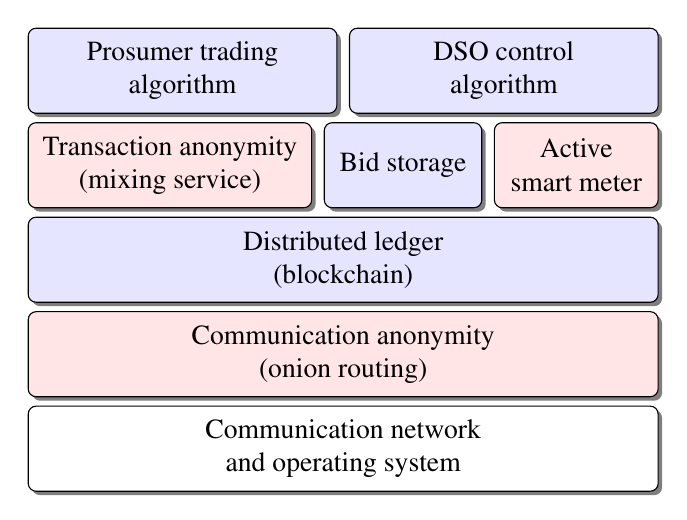
\begin{tikzpicture}[x=8cm, y=1.2cm,
  nodeStyle/.style={rounded corners=0.1cm, drop shadow={shadow xshift=0.05cm, shadow yshift=-0.05cm, fill=black}}
]
\draw [nodeStyle, fill=white]   (0, 0) rectangle    (1, 0.9) node [midway, align=center] {Communication network\\and operating system};

\draw [nodeStyle, fill=red!10]  (0, 1) rectangle    (1, 1.9) node [midway, align=center] {Communication anonymity\\(onion routing)};

\draw [nodeStyle, fill=blue!10] (0, 2) rectangle    (1, 2.9) node [midway, align=center] {Distributed ledger\\(blockchain)};

\draw [nodeStyle, fill=red!10]  (0,    3) rectangle (0.45, 3.9) node [midway, align=center] {Transaction anonymity\\(mixing service)};
\draw [nodeStyle, fill=blue!10] (0.47, 3) rectangle (0.72, 3.9) node [midway, align=center] {Bid storage};
\draw [nodeStyle, fill=red!10 ] (0.74, 3) rectangle (1,    3.9) node [midway, align=center] {Active\\smart meter};

\draw [nodeStyle, fill=blue!10] (0,    4) rectangle (0.49, 4.9) node [midway, align=center] {Prosumer trading\\algorithm};
\draw [nodeStyle, fill=blue!10] (0.51, 4) rectangle (1,    4.9) node [midway, align=center] {DSO control\\algorithm};
\end{tikzpicture}
\caption{High-level architecture of the proposed solution. Components marked red are introduced to provide privacy in a safe and secure manner. Components marked in blue are typical elements of a decentralized transactive microgrid.}
\label{fig:softwareArchitecture}
\end{figure}

\begin{figure*}[h]
\center
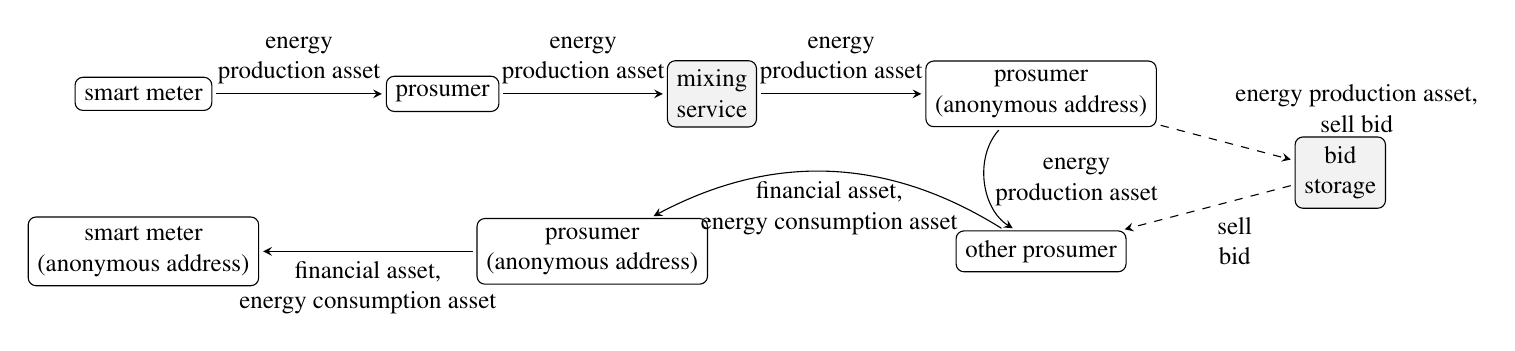
\begin{tikzpicture}[x=3.8cm, y=2cm, font=\small,
  system/.style={draw, align=center, rounded corners=0.1cm, fill=black!5},
  entity/.style={draw, align=center, rounded corners=0.1cm},
  asset/.style={midway, align=center},
  transfer/.style={->, >=stealth, shorten <=0.05cm, shorten >=0.05cm},
]
%\node[entity] (smartmeter) at (0.75, 0.5) {smart\\meter};
%\node[entity] (prosumer1) at (1.25, 1) {prosumer};
%\node[system] (mixing1) at (2, 1) {mixing\\service};
%\node[entity] (prosumer2) at (3, 1) {prosumer\\(alternative address)};
%\node[system] (bidstorage) at (4, 1) {bid\\storage};
%\node[entity] (partner) at (4, 0) {other prosumer};
%\node[entity] (prosumer3) at (3, 0) {prosumer\\(alternative address)};
%\node[system] (mixing2) at (2, 0) {mixing\\service};
%\node[entity] (prosumer4) at (1.25, 0) {prosumer};
\node[entity] (smartmeter) at (0, 1) {smart meter};
\node[entity] (prosumer1) at (1, 1) {prosumer};
\node[system] (mixing1) at (1.9, 1) {mixing\\service};
\node[entity] (prosumer2) at (3, 1) {prosumer\\(anonymous address)};
\node[system] (bidstorage) at (4, 0.5) {bid\\storage};
\node[entity] (partner) at (3, 0) {other prosumer};
\node[entity] (prosumer3) at (1.5, 0) {prosumer\\(anonymous address)};
\node[entity] (smartmeter2) at (0, 0) {smart meter\\(anonymous address)};

%\draw[transfer] (smartmeter) -- node [asset, above left] {energy\\production asset} (prosumer1);
%\draw[transfer] (prosumer1) -- node [asset, above] {energy\\production asset} (mixing1);
%\draw[transfer] (mixing1) -- node [asset, above] {energy\\production asset} (prosumer2);
%\draw[transfer, dashed] (prosumer2) -- node [asset, above] {energy production asset,\\sell bid} (bidstorage);
%\draw[transfer, dashed] (bidstorage) -- node [asset, right] {sell\\bid} (partner);
%\draw[transfer, bend right=15] (partner) to node [asset, below] {financial asset,\\energy\\consumption asset} (prosumer3);
%\draw[transfer, bend right=7.5] (prosumer2) to node [asset, above right] {energy\\prod. asset} (partner);
%\draw[transfer] (prosumer3) -- node [asset, below] {financial asset,\\
%energy consumption asset} (mixing2);
%\draw[transfer] (mixing2) -- node [asset, below] {financial asset,\\energy consumption asset} (prosumer4);
%\draw[transfer] (prosumer4) -- node [asset, below left] {financial\\asset} (smartmeter);

\draw[transfer] (smartmeter) -- node [asset, above] {energy\\production asset} (prosumer1);
\draw[transfer] (prosumer1) -- node [asset, above] {energy\\production asset} (mixing1);
\draw[transfer] (mixing1) -- node [asset, above] {energy\\production asset} (prosumer2);
\draw[transfer, dashed] (prosumer2) -- node [asset, above right] {energy production asset,\\sell bid} (bidstorage);
\draw[transfer, dashed] (bidstorage) -- node [asset, below right] {sell\\bid} (partner);
\draw[transfer, bend right=30] (partner) to node [asset, below] {financial asset,\\energy consumption asset} (prosumer3);
\draw[transfer, bend right=50] (prosumer2) to node [asset, right] {energy\\production asset} (partner);
\draw[transfer] (prosumer3) -- node [asset, below] {financial asset,\\
energy consumption asset} (smartmeter2);
\end{tikzpicture}
\caption{Simplified overview of the flow of assets from the perspective of a prosumer who sells energy production. Note that in order to prevent de-anonymization, a prosumer should use multiple addresses for mixing and multiple rounds of mixing.}
\end{figure*}

\subsection{Timing}
The ability to specify points or intervals in time is crucial.
For example, control signals specify how the load should change at certain points in time, energy trades specify when energy will be consumed or produced, etc.
To facilitate processing signals and transactions, we divide time into fixed-length intervals, and specify points or periods in time using these discrete timesteps.
The length of the time interval is determined by mapping the timing assumptions of the power system to our platform.
%In our implementation, 
For example, the default length of the time interval may be 4 seconds, which corresponds to how frequently the control signal of the DSO typically changes.

\subsection{Services}

Here, we describe three services that must be implemented for our solution: communication anonymity, mixing service for transaction anonymity, and anonymous bid storage for bidding anonymity.

\subsubsection{Communication Anonymity}
Firstly, we must provide an anonymous communication layer, on which we can build an anonymous trading platform.
Without this communication layer, bids and transactions could be easily de-anonymized based on the network identifiers of the sources (e.g., IP or MAC addresses).

We can employ well-known and widely used techniques for anonymous communication, such as \emph{onion routing}.
To build an onion network, the smart meters, inverters, and other devices can act as onion routers, and the list of onion routers in a microgrid can be published on a private blockchain.
In our first implementation, we can use the free and open-source Tor software with private Directory Authorities.
% ritter.vg: "run your own tor network"
% https://ritter.vg/blog-run_your_own_tor_network.html

\subsubsection{Transaction Anonymity}
We must provide prosumers with the ability to create and publish transactions anonymously.
More specifically, prosumers should be able to purchase or sell energy without revealing their identity; however, these transaction must also be verifiable and enforceable.

We may achieve this goal using multiple approaches for blockchain transaction anonymity:
\begin{itemize}
\item Mixing services (also known as tumblers) mix potentially identifiable assets on a blockchain with others, thereby preventing tracing individual assets back to their original source. 
In our case, assets to be mixed include virtual balances of fiat currencies as well as energy production and consumption.
\item Cryptographic anonymity for transactions is provided, for example, by Zerocoin~\cite{miers2013zerocoin}. Similarly to mixing service, Zerocoin can prevent tracing assets on a blockchain.
\end{itemize}
Using the above techniques, we can enable prosumers to trade energy anonymously (i.e., without revealing their true identities), but at the same time prevent them from altering their energy or financial balances without a valid transaction.

However, we must also ensure that 1) smart meters know the amount of energy purchased or sold by their prosumer and 2) prosumers cannot purchase or sell more energy than their capacity.
To satisfy both of these constraints, all energy trades must start with the prosumer withdrawing a certain amount of energy production or consumption from its smart meter:
\begin{itemize}
\item If a prosumer wishes to sell energy, it must first obtain an energy asset from its smart meter using a blockchain transaction.
This transaction must be signed by the smart meter, which enables the smart meter to 1) keep track of the amount of energy traded by the prosumer as well as to 2) enforce safety requirements by limiting the amount of energy that can be withdrawn.
\item If a prosumer wishes to buy energy, it must first obtain an energy consumption asset from its smart meter in a way similar to obtaining an energy production asset.
\end{itemize}

\subsubsection{Bidding Anonymity}
Finally, we must provide prosumers with the ability to publish energy buy and sell bids anonymously.
To this end, we create a storage for anonymous bids that is readable by all the prosumers in the microgrid.
Any prosumer may submit a bid to this storage; however, in order to do so, they must provide a zero-knowledge proof of owning the assets that are to be traded:
\begin{itemize}
\item To submit an energy sell bid, the prosumer must prove that it owns an energy production asset on the chain.
\item To submit an energy buy bid, the prosumer must prove that it own an energy consumption asset as well as financial assets on the chain.
\end{itemize}


\subsection{Transaction Types}

Before we can discuss transaction types, we must first define the three assets that these transactions may transfer.

An \emph{energy production asset} (EPA) is defined by
\begin{compactitem}
\item \field{power}: non-negative amount of power to produced (for example, measured in watts).
\item \field{start}: first time interval in which energy is to be produced. 
\item \field{end}: last time interval in which energy is to be produced.
\end{compactitem}
An \emph{energy consumption asset} (ECA) is defined by the same fields; however, for this asset, the fields define consumption instead of production.
Finally, a \emph{financial asset} (FA) is defined by a single non-negative field \field{amount}, which can be denominated in either a fiat currency (e.g., US dollars) or a cryptocurrency.

\subsubsection{Energy and Financial Transactions}

Energy and financial transactions transfer energy and financial asset from one address to another.
Prosumers use these transactions for multiple purposes: to trade energy by exchanging assets with other prosumers, to prove to the bid storage that they have production or consumption capacity, to hide their identity by transferring assets to and from mixing services, and to deposit assets at their smart meter.
%
An energy and financial transaction contains the following fields:
\begin{compactitem}
\item List of EPA inputs, each of which is defined by:
\begin{compactitem}
\item \field{out}: EPA output from a previous transaction,
\item \field{sig}: signature for this output.
\end{compactitem}
\item List of ECA inputs, each of which is defined by:
\begin{compactitem}
\item \field{out}: ECA output from a previous transaction,
\item \field{sig}: signature for this output.
\end{compactitem}
\item List of FA inputs, each of which is defined by:
\begin{compactitem}
\item \field{out}: FA output from a previous transaction,
\item \field{sig}: signature for this output.
\end{compactitem}
\item List of EPA outputs, each of which is defined by:
\begin{compactitem}
\item an EPA and an address to which it is transferred.
\end{compactitem}
\item List of ECA outputs, each of which is defined by:
\begin{compactitem}
\item an ECA and an address to which it is transferred.
\end{compactitem}
\item List of FA outputs, each of which is defined by:
\begin{compactitem}
\item an FA and an address to which it is transferred.
\end{compactitem}
\end{compactitem}

An energy and financial transaction is valid if the following three conditions hold.
\begin{compactitem}
\item None of the outputs referenced by the inputs have been spent by a transaction that has been recorded on the ledger.
\item All of the signatures are valid.
\item For each asset type (and for each timestep), the sum of inputs and outputs is the same.
For example, in the case of energy production assets, the condition is:
\begin{align}
\forall t: & \sum_{out \in \text{EPA outputs}} out.\mathtt{power} \cdot 1_{\left\{out.\mathtt{start} \leq t \leq out.\mathtt{end}\right\}} \nonumber \\
& = \sum_{in \in \text{EPA inputs}} in.\mathtt{out}.\mathtt{power} \cdot 1_{\left\{in.\mathtt{out}.\mathtt{start} \leq t \leq in.\mathtt{out}.\mathtt{end}\right\}} ,
\end{align}
where $1_x$ is equal to $1$ if $x$ is true, and it is $0$ otherwise.
%\begin{equation}
%\forall t: \sum_{out \in \left\{out' \middle| out' \in \text{ EPA outputs} \wedge out'.EPA.start \leq t \leq out'.EPA.end\right\}} out.EPA.Power = \sum_{in \in \left\{in' \middle| in' \in \text{ EPA inputs} \wedge in'.EPA.start \leq t \leq in'.EPA.end\right\}} in.EPA.Power .
%\end{equation}
\end{compactitem}
If a transaction submitted to the ledger is valid, it will be permanently recorded.

\subsubsection{Smart-Meter Transactions}

Prosumers use smart-meter transactions to withdraw energy and financial assets from their own smart meters, before they engage in energy trading.
%
A smart-meter transaction contains the following fields:
\begin{compactitem}
\item List of EPA outputs, each of which is defined by:
\begin{compactitem}
\item an EPA and an address to which it is transferred.
\end{compactitem}
\item List of ECA outputs, each of which is defined by:
\begin{compactitem}
\item an ECA and an address to which it is transferred.
\end{compactitem}
\item List of FA outputs, each of which is defined by:
\begin{compactitem}
\item an FA and an address to which it is transferred.
\end{compactitem}
\item \field{id}: Identifier of the smart meter.
\item \field{sig}: Smart meter's signature over the transaction.
\end{compactitem}

A smart-meter transaction is valid if the following two conditions hold:
\begin{compactitem}
\item The smart meter identified in the transaction has been authorized by a regulatory transaction that has been recorded on the ledger.
\item The smart meter's signature is valid.
\end{compactitem}
\todo{To address malfunctioning or compromised smart meters, we could also impose a limit on withdrawals.}

\subsubsection{Regulatory Transactions}

The DSO uses regulatory transactions to authorize or ban smart meters and to control the microgrid load through setting a price policy.
Since these transactions provide a diverse set of functionality, they are divided into two types.

\paragraph{Authorize or Ban Smart Meters}
The DSO uses these transactions to manage the set of authorized smart meters in the microgrid.
Whenever a new smart meter is installed, the DSO notifies the members of the microgrid using a regulatory transaction.
Similarly, whenever a smart meter is deactivated (e.g., because service is stopped or it is believed to be malfunctioning or compromised), the DSO notifies the members of the microgrid using a regulatory transaction.
These transactions contain the following fields:
\begin{compactitem}
\item List of smart meters to be authorized, each of which is defined by:
\begin{compactitem}
\item \field{id}: Identifier of the smart meter.
\item \field{pubkey}: Public key of the smart meter.
\end{compactitem}
\item List of smart meters to be banned, each of which is given using its identifier.
\item \field{time}: Timestep in which smart meters are authorized and banned.
\item \field{sig}: DSO's signature over the transaction.
\end{compactitem}

A regulatory transaction of this type is valid if the following two conditions hold:
\begin{compactitem}
\item The timestep specified in the transaction is in the future.
\item The DSO's signature is valid.
\end{compactitem}

\paragraph{Price Policy}


\section{Analysis}
\label{sec:analysis}

Here, we present a semi-formal analysis of the proposed solution, and show that it satisfies the security, safety, and privacy requirements.

\subsection{Security}

\subsection{Safety}

\subsection{Privacy}

Due to the communication anonymity and mixing services, members of a microgrid can see only the amount of energy and financial assets withdrawn by a prosumer.
Since all trading transactions are anonymous, the amount of assets traded by the prosumer will not be publicly known.
In case a prosumer does not wish to trade, it can anonymously deposit its assets to a random address that was freshly generated by its smart meter.
Note that even if a prosumer does not wish to trade, it should always withdraw and mix assets; otherwise, the lack of withdrawal would leak information.

As for the DSO, it can receive the same information from the smart meter as in a non-transactive grid (i.e., amount of energy produced and consumed).
\todo{Also knows financial amounts, but those are necessary for billing.}
Since trading is anonymous, it does not receive any further information.

In fact, we can provide an even higher-level of privacy.
Since price policies are recorded on the ledger, which the smart meters may read, the smart meters can calculate the prosumer's monthly bill, and send only this single financial amount to the DSO each month.
Meanwhile, the DSO can still obtain current and future load information from the bid storage and from the trades recorded on the ledger.


\section{Related Work}
\label{sec:related}

\subsection{Smart Grid and Meter Privacy}

% http://ieeexplore.ieee.org/abstract/document/5054916/
McDaniel and McLaughlin discuss privacy challenges in smart grids~\cite{mcdaniel2009security}.

% https://arxiv.org/pdf/1108.2234.pdf
% https://pdfs.semanticscholar.org/cdf8/a5b6256823bca38a1d2347ab36f8e4a2ca94.pdf
Rajagopalan et al.\ use tools from information theory to present a framework, which abstracts both the privacy and the utility requirements of smart meter data~\cite{rajagopalan2011smart,sankar2013smart}. Their framework leads to a novel privacy-utility tradeoff problem with minimal assumptions. %, which is tractable.

% http://www.comm.toronto.edu/~akhisti/sm.pdf
Varodayan and Khisti study using rechargeable battery for partially protecting the privacy of information contained in a household's electrical load profile~\cite{varodayan2011smart}.
They show that stochastic battery policies may leak 26\% less information than a best-effort policy, holds the output load constant whenever possible.

% https://www.researchgate.net/profile/Georgios_Kalogridis/publication/224189766_Smart_Grid_Privacy_via_Anonymization_of_Smart_Metering_Data/links/541169510cf2b4da1bec4193.pdf
Efthymiou and Kalogridis describe a method for securely anonymizing frequent electrical metering data sent by a smart meter~\cite{efthymiou2010smart}. 
Their approach is based on the observation that frequent metering data may be required by an energy distribution network for operational reasons, but it may not necessarily need to be attributable to a specific smart meter.
The authors describe a method that provides a third-party escrow mechanism for authenticated anonymous meter readings, which are difficult to associate with particular smart meter.

% https://arxiv.org/pdf/1305.0735.pdf
Tan et al.\ study privacy in a smart metering system from an information theoretic perspective in the presence of energy harvesting and storage units~\cite{tan2013increasing}. 
They show that energy harvesting provides increased privacy by diversifying the energy source, while a storage device can be used to increase both energy efficiency and privacy. 
They show that there exists a trade-off between the information leakage rate and the wasted energy rate, and study the impact of the energy harvesting rate and the size of the storage device on this trade-off.

\subsection{Blockchain Technology}

Microsoft offers Blockchain as a Service (BaaS) on Azure.
Project Bletchley is Microsoft's architectural approach to building an Enterprise Consortium Blockchain Ecosystem, introducing two new concepts: blockchain middleware and cryptlets~\cite{gray2016introducing}.

Hyperledger Fabric is a platform for distributed ledger solutions, which was designed to support pluggable implementations of different components~\cite{hyperledger2017fabric}.

Interledger is a protocol for payments across payment systems, which enables anyone with accounts on two ledgers to create
a connection between them~\cite{thomas_protocol}.

Bitcoin Lightning Network is decentralized system, in which transactions are sent over a network of micropayment channels whose transfer of value occurs off-blockchain~\cite{poon2016bitcoin}.

\url{https://geli.net/residential/}
\url{https://www.greentechmedia.com/articles/read/geli-raises-7m-to-take-energy-storage-software-to-the-next-level}



\section{Conclusion}
\label{sec:concl}



% BALANCE COLUMNS
\balance{}

% REFERENCES FORMAT
% References must be the same font size as other body text.
\bibliographystyle{SIGCHI-Reference-Format}
\bibliography{references}

\end{document}

